\documentclass[a4paper,12pt]{report}

\usepackage[francais]{babel}
\usepackage[T1]{fontenc}
\usepackage[latin1,utf8]{inputenc}
\usepackage{soul}
\usepackage{lmodern}
\usepackage{amsmath}
\usepackage{amssymb}
\usepackage{mathrsfs}
\usepackage{amsmath}
\usepackage{amsfonts}
\usepackage{amssymb}
\usepackage{graphics}
\usepackage{pgf,tikz}
\usepackage{multirow}
\usepackage{listings}
\usepackage{algorithm}
\usepackage{algorithmic}
\usepackage{graphicx}

\setlength{\parindent}{0cm}
\setlength{\parskip}{1ex plus 0.5ex minus 0.2ex}
\newcommand{\hsp}{\hspace{20pt}}
\newcommand{\HRule}{\rule{\linewidth}{0.5mm}}

\begin{document}

\begin{titlepage}
  \begin{sffamily}
  \begin{center}

    \textsc{ Université Pierre et Marie Curie \\[1cm] \huge Résolution de problèmes}\\[6cm]

    \textsc{\huge \bfseries Résolution de Mots Croisés par un CSP.}\\

    % Title
    \HRule \\[0.4cm]

~~\\
~~\\
    % Author and supervisor
    \begin{minipage}{0.4\textwidth}
      \begin{center} \large
        Renaud \textsc{ADEQUIN}\\
        Nadjet \textsc{BOURDACHE}\\
      \end{center}
    \end{minipage}

    \vfill

    % Bottom of the page
    {\large 04/04/2016}

  \end{center}
  \end{sffamily}
\end{titlepage}

\section*{1. Modélisation par un CSP et résolution}
\begin{enumerate}
\item Pour résoudre ce problème, on propose une modélisation qui consiste à associer une variable à chaque mot de la grille. Les mots de la grille étants numérotés dans l'odre de leurs apparition dans la grille (d'abord les mots horizontaux puis les verticaux). On définit ensuite un ensemble de contraintes pour vérifier la cohérence de la grille générée.

~~\\
\textbf{Variables:}


Pour \textit{m} mots, on a \textit{m} variables : \textit{$Mot_i$} , $\forall$ $i$  $\in$ $\{1, ... , m \}$.

~~\\
\textbf{Domaine:}


Chaque mot de la grille doit appartenir au dictionnaire considéré, notons le $Dict$.
\begin{center}
D(\textit{$Mot_i$}) $=$ $\{ X \in$ $Dict$  : $|X|$ = $|Mot_i|$ $\}$, $\forall$  $i$ $\in$ $\{1, ... , m \}$ .
\end{center}

~~\\
\textbf{Contraintes:}\\
\begin{itemize}
\item Pour toute paire de mots \textit{Mot$_i$} et \textit{Mot$_j$} qui se croisent aux positions \textit{p} pour \textit{Mot$_i$} et \textit{q} pour \textit{Mot$_j$}, on définit la contrainte:
$$\textit{Mot}_i [p]\ =\  \textit{Mot}_j [q] .$$ 

\item Pour modéliser le fait qu'un même mot ne peut apparaître plus d'une fois dans la grille, il suffit d'ajouter la contrainte:
$$ \textit{AllDiff}\ (\textit{Mot}_1, \textit{Mot}_2, \cdots , \textit{Mot}_m)  $$\\
\end{itemize}

\item D'un point de vue algorithmique, nous avons mis en œuvre une classe "Grille". Chaque objet de cette classe représente une instance de mots croisés, et contient une taille, un dictionnaire, une liste de tous les mots de la grille ayant une taille supérieure à 1 ainsi qu'une liste de cases noires.\\
On pourra à partir d'un objet de cette classe, initialiser une grille à partir d'un fichier texte contenant une grille ou en générer une aléatoirement et la sauvegarder dans un fichier après résolution.\\

\item Les algorithmes AC3 et FC ont été développés tel qu'ils ont été définis en cours. \\

\item En revanche, pour le Conflict BackJumping, afin d’améliorer la résolution, nous avons:
\begin{itemize}
\item Effectuer une arc-consistance sur les mots de la grille pour réduire les domaines avant de lancer l'algorithme.
\item Nous avons aussi ajouter un Check Forward avant l'appel récursif, ce qui nous permet d'éviter des appels inutiles et d'améliorer encore le temps de résolution des grilles les plus grandes.\\
\end{itemize}

\item Afin d'améliorer les trois algorithmes, nous avons utilisé une structure d'arbre pour sauvegarder et manipuler les dictionnaires et les domaines des différentes variables.\\
 Cette structure permet un parcours rapide du dictionnaire pour l'initialisation des domaines, et surtout, elle permet d’accélérer les algorithmes de filtrage, puisqu'elle peut permettre d'éliminer plusieurs mots d'un domaine en supprimant des sous arbres de ce dernier, nous évitant ainsi de devoir parcourir et tester chaque mot du domaine.\\
\end{enumerate}

\section*{2. Expérimentations}
\begin{enumerate}
\item Pour le filtrage par AC3, les résultats obtenus pour les différentes grilles sont représentés sur les graphiques ci-dessous.

On voit clairement que le temps du filtrage augmente exponentiellement avec la taille des dictionnaires utilisés. Ce qui se justifie par une plus grande taille du domaines des variables, et donc par plus de valeurs pour lesquels on vérifiera la consistance.

On remarque surtout, que plus la grille contient de mots, plus les temps croissent rapidement lorsqu'on augmente la taille des dictionnaires. Ceci est du au fait qu'il y ai plus de variables, et donc plus de contraintes à vérifier et plus de domaines qui croissent lorsque la taille augmente.
\begin{table*}[!h]
\begin{center}
\begin{tabular}{|c|}
\hline
 {Filtrage par AC3} \\
\hline
\hline
  Grille A\\
\hline   
   \\
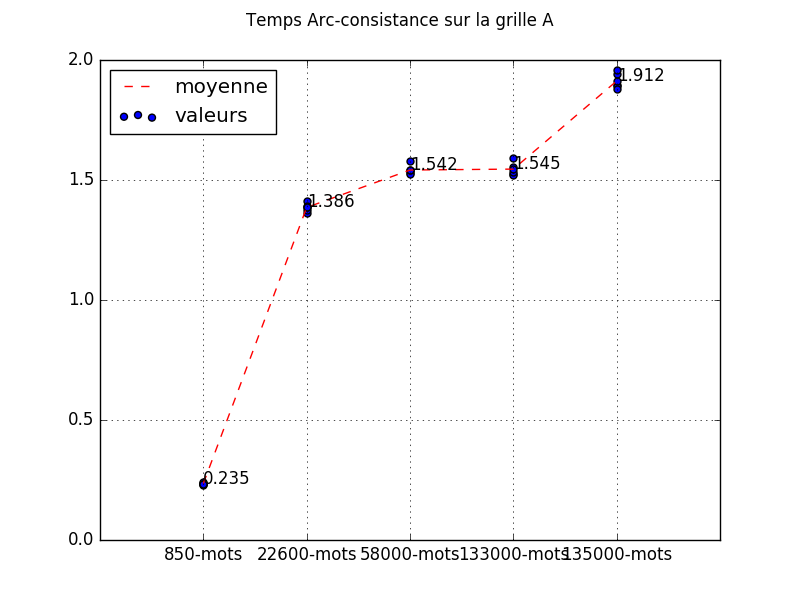
\includegraphics[width=7.5cm]{AC3_A.png}  \\
\hline
Grille B \\
\hline 
\\
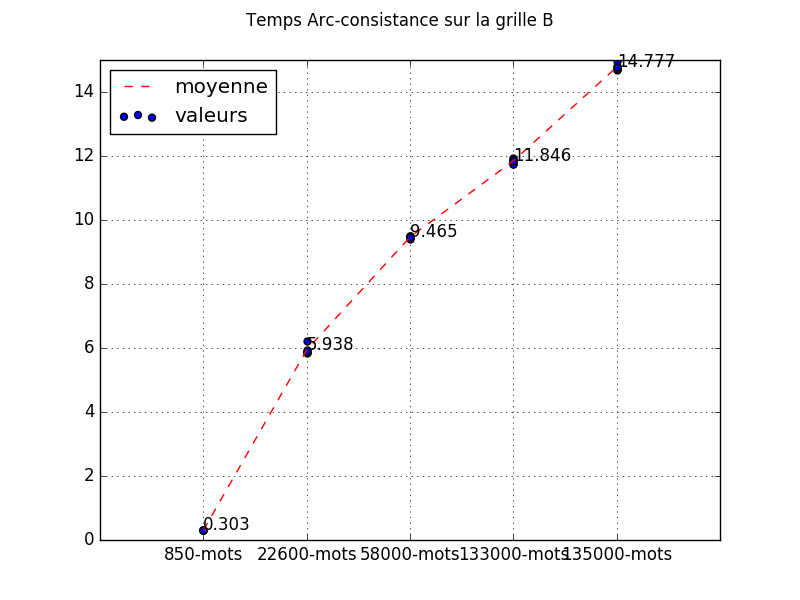
\includegraphics[width=7.5cm]{AC3_B.png} \\
\hline
Grille C\\
\hline
  \\
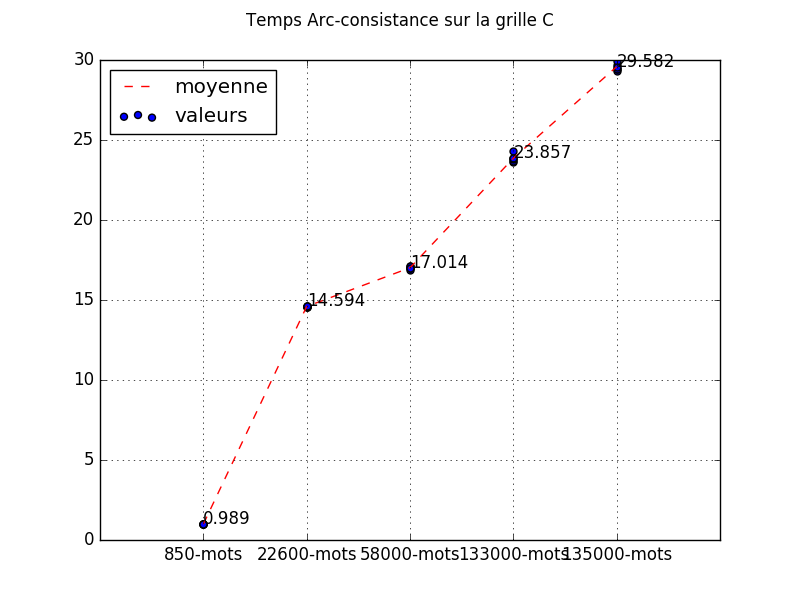
\includegraphics[width=7.5cm]{AC3_C.png} \\
\hline

\end{tabular}
\end{center}
\end{table*}


\begin{table*}[!h]
\begin{center}
\begin{tabular}{|c|}
\hline
 {RAC avec Forward Checking sans AC3 préalable} \\
\hline
\hline
  Grille A\\
\hline   
   \\
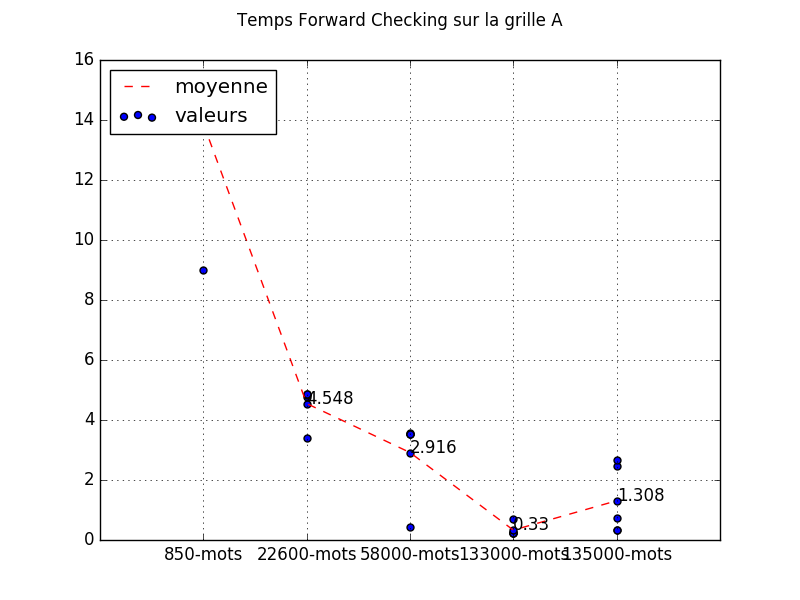
\includegraphics[width=7.5cm]{FC_A.png}  \\
\hline
Grille B \\
\hline 
\\
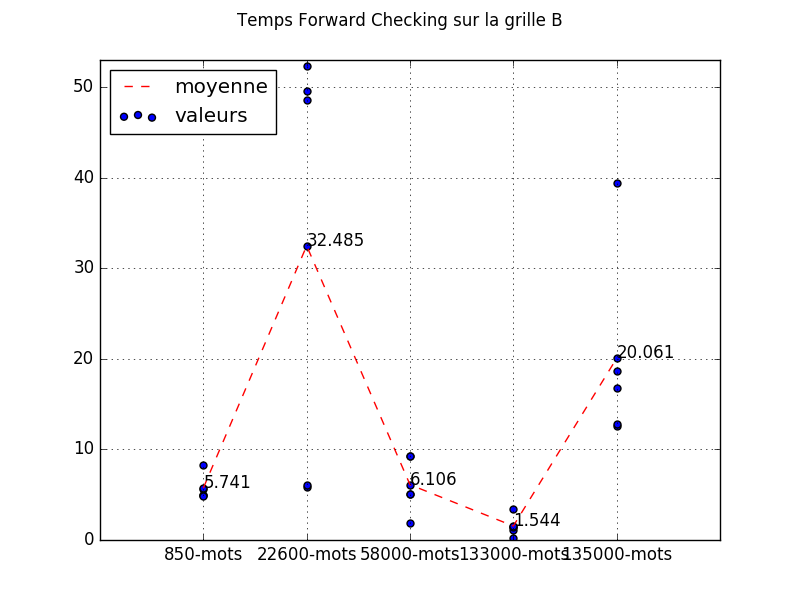
\includegraphics[width=7.5cm]{FC_B.png} \\
\hline
Grille C\\
\hline
  \\
 \\
\hline

\end{tabular}
\end{center}
\end{table*}

\begin{table*}[!h]
\begin{center}
\begin{tabular}{|c|}
\hline
 {RAC avec Forward Checking et AC3 préalable} \\
\hline
\hline
  Grille A\\
\hline   
   \\
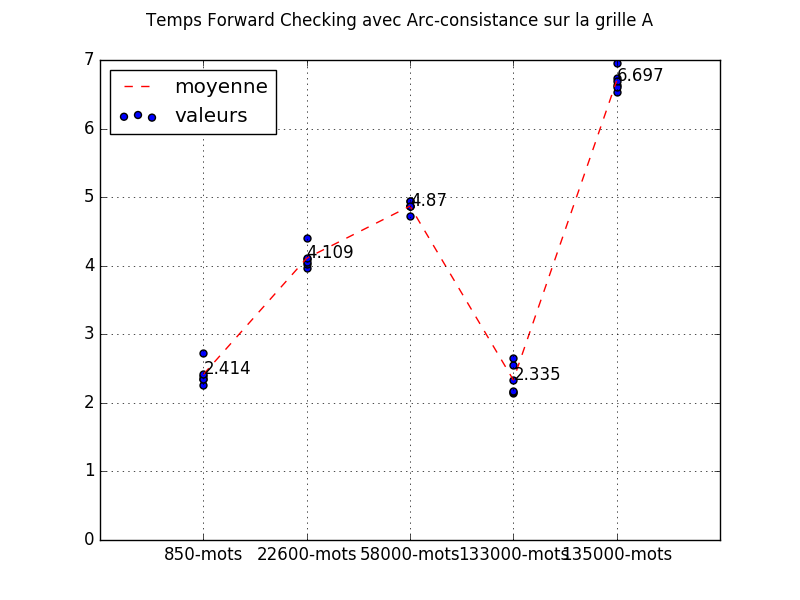
\includegraphics[width=7.5cm]{FC_AC3_A.png}  \\
\hline
Grille B \\
\hline 
\\
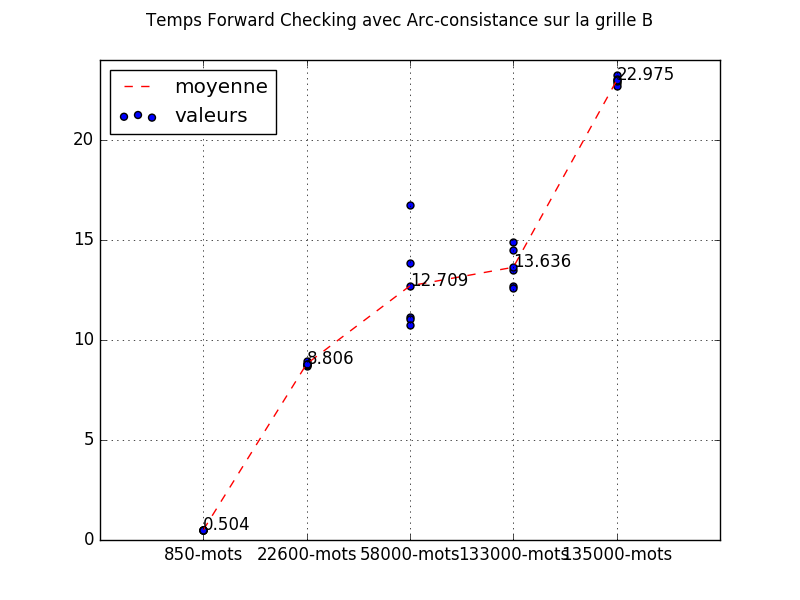
\includegraphics[width=7.5cm]{FC_AC3_B.png} \\
\hline
Grille C\\
\hline
  \\
 \\
\hline

\end{tabular}
\end{center}
\end{table*}



\end{enumerate}



\end{document}